\documentclass[czech,BP]{thesiskiv}

\author{Jan Kohlíček}
\declarationmale

\title{Skladové hospodářství pomocí RFID a RaspberryPi}

\abstracttexten{The text of the abstract (in English). It contains the English translation of the thesis title and a short description of the thesis.}

\abstracttextcz{Text abstraktu (česky). Obsahuje krátkou anotaci (cca 10 řádek) v češtině. Budete ji potřebovat i při vyplňování údajů o bakalářské práci ve STAGu. Český i anglický abstrakt by měly být na stejné stránce a měly by si obsahem co možná nejvíce odpovídat (samozřejmě není možný doslovný překlad!).
}

\usepackage[nottoc,notlot,notlof]{tocbibind}
\usepackage[pdftex]{graphicx}
\usepackage[pdftex]{hyperref}
\hypersetup{colorlinks=true,
  unicode=true,
  linkcolor=black,
  citecolor=black,
  urlcolor=black,
  bookmarksopen=true}
\usepackage[numbers,sort&compress]{natbib}
\usepackage{color}
\usepackage{xcolor}
\usepackage{multirow}
\usepackage{tabularx}
\usepackage{lipsum}

\begin{document}

\maketitle
\tableofcontents


\chapter{Úvod}

	
\chapter{Skladové hospodářství}
Skladové hospodářství je nedílnou součástí logistického systému. Sklady mají za úkol přijímat zásoby, uchovávat a vydávat je a provádět potřebné skladové manipulace. Skladové hospodářství má v podnicích návaznost na téměř všechny ostatní úseky. Hlavním úkolem skladu je ekonomické sladění rozdílně dimenzovaných toků v podniku, a to tak, aby bylo dosaženo synergického efektu.\cite{vitek2007skladove}


\section{Současný skladový systém}
Pod tímto pojmem si můžeme představit systém pro evidenci skladu resp. skladovaných zásob (příjem  a  výdej  materiálu), systém pro účtování zásob a jejich objednávek nebo systém pro inventarizaci. Můžeme tedy říci, že skladový systém je systém pro správu ekonomických operací nad skladem.\cite{hron2014skladovy}


\section{Skladový systém s RFID}

\subsection{Rychlé načtení údajů}
\texttt{RFID} čip má oproti etiketě s čárovým kódem dvě hlavní výhody - rychlost čtení a nepřímou viditelnost čtecího zařízení na čip. Současné standardy \texttt{UHF RFID} čipů umožňují načíst najednou až 1000 čipů za sekundu, tato hodnota se však s příchodem novějších a výkonnějších zařízení bude zvyšovat. \texttt{RFID} čtecí zařízení nepotřebuje mít přímou viditelnost na jednotlivé čipy, čtení i zápis probíhá bezdrátově a to do vzdálenosti cca 15 m u pasivních čipů a až 100 m u aktivních čipů.\cite{dolevcek2010identifikace}
\\
Například paletový přepravník tak může projet celým \texttt{RFID} čtecím portálem a v jeden čas dojde k současnému načtení všech čipů na paletě, tím se dosáhne zrychlení procesu příjmu, výdeje, přesunu a inventarizace produktu.\cite{dolevcek2010identifikace}

\subsection{Odstranění chyb obsluhy}
\texttt{RFID} čipy společně se čtecím zařízením vylučují možnost vzniku chyby obsluhy, které vzniknou například tím, že obsluha načte pouze část \texttt{čárových kódů} na paletě.\cite{dolevcek2010identifikace}

\subsection{Zápis údajů o zboží během celého logistického pohybu}
\texttt{RFID} čip má oproti etiketě s \texttt{čárovým kódem} hlavní výhodu v tom, že do čipu lze informace i zapisovat a nejenom číst, jak je to v případě \texttt{čárového kódu}. Tato vlastnost bude v budoucnosti klíčová a rozhodne v mnoha odvětvích pro úplnou náhradu \texttt{čárového kódu} \texttt{RFID} čipem. Do čipu lze navíc informace zapisovat a měnit opakovaně, lze takto do každého produktu zapsat datum výroby a poté také připsat jednotlivé logistické zápisy, které vznikají po celou dobu cesty produktu.\cite{dolevcek2010identifikace}

\subsection{Přesná evidence spotřebitelských jednotek}
V současnosti při samotném logistickém procesu obsluha načte \texttt{čárový kód} palety, ale již není schopna ověřit, zda je na paletě správný počet kartónů a správný počet produktů. Jediným řešením by bylo paletu rozebrat a postupně načíst všechny \texttt{čárové kódy}. \texttt{RFID} čtecí portál však načte najednou všechny RFID čipy na paletě nalezené. Navíc dle typu čipu dokáže vyhodnotit počet \texttt{RFID} čipů kartónů i počet RFID čipů samotných produktů.\cite{dolevcek2010identifikace}

\subsection{Odolnost RFID čipů}
Etiketa s \texttt{čárovým kódem} podléhá teplotním a povětrnostním vlivům a následně dochází k poškození etikety. Je tomu hlavně proto, že je nutné etikety s \texttt{čárovým kódem} umisťovat tak, aby je bylo možné načíst čtecím zařízením a tudíž zvenku. \texttt{RFID} čip je umístěn uvnitř produktu nebo balení a tím je odolný jak proti teplotě, vodě i povětrnosti. V současné době na trhu již existují \texttt{RFID} čipy, které navíc mohou obsahovat čidla - například pro měření vlhkosti nebo teploty. \cite{dolevcek2010identifikace}


\subsection{Optimalizace skladových zásob}
Představme si tak obvyklou záležitost, jakou je příjem materiálu (zboží) a jeho naskladnění. Tato operace dnes probíhá v mnoha společnostech po jednotlivých kusech (logistických jednotkách), a tak se také informace dostávají do informačního systému (se zpožděním).
Celá došlá zásilka je načtena \texttt{RFID} čtečkami během několika sekund a tato informace (násobně větší objem) se přenáší do informačního systému, který dosud nebyl na tento způsob zpracování informací připraven. Výsledkem tohoto naskladnění je okamžitá informace o stavu našeho skladu, a dramatické zrychlení jejího získání. Vybavíme-li stejnou technologií také výrobu ve společnosti, získáme tak stejné informace z jednotlivých částí výroby (stav výroby, průběžné zásoby na pracovišti). 
Dramatické zrychlení sběru informací v rámci logistiky (výroby) umožňuje daleko lepší plánování zásob společnosti. Pokud máme plán výroby a stavy zásob, tak zásoby, které máme na skladě můžeme odpovědně řídit ne z hlediska \texttt{Q (množství)}, ale z hlediska 
\texttt{T (času)}. Tím se zcela zásadním způsobem zjednodušuje systém predikce objednávek a otevírá se velký prostor pro optimalizaci skladových zásob - úspory na vázaném kapitálu.\cite{dolevcek2010identifikace}



\section{Popis systému RFID-RMS}

Systém \texttt{RFID-RMS} se používá pro poskytovatele logistických služeb ke zlepšení skladových operací pomocí sledování a optimalizace využitých zdrojů. \texttt{RFID-RMS} využívá mobilní technologie k přesnému určení lokalizace, sledování a řízení zdrojů v prostředí skladu. Architektura systému \texttt{RFID-RMS} se skládá ze dvou částí, které přispívají k rozhodovacímu procesu v oblasti řízení zdrojů. První část je \texttt{frontend}, obsahující dva moduly pro sběr dat, a to modul pevných logistických dat a modul proměnných logistických dat. Tyto dva moduly obsahují dva různé typy \texttt{RFID tagů} pro ulehčení přenosu a ukládání logistických dat. Druhá část je \texttt{backend}, který obsahuje modul sledování zdrojů, modul řízení zdrojů a datového úložiště. Primární funkcí této části je provádět řízení zdrojů, sledování zdrojů, hodnotit využití zdrojů, výběr nejvhodnější trasy, údržba a kontrola provozu.\cite{chow2006design}

\subsection{Sběr dat}

\texttt{Modul pevných logistických dat} používá nízkoúrovňové \texttt{radiové} signály pro výměnu dat mezi pasivními \texttt{tagy} a čtečkou. Pasivní \texttt{tag} se skládá z \texttt{integrovaného obvodu} pro uložení identity položek a dalších informací. Jak je znázorněno na obrázku \ref{fig:passive}, pasivní značka je připojena na položky, jako jsou palety, obaly atd. Čtečky tagů s pevnou pozicí antén jsou namontovány do konstrukce jako jsou dveře, vstupní brána nebo integrované do vysokozdvižných vozíků a ostatního vybavení. Obsahuje-li více antén, dokáží v rámci svého rozsahu najednou rozpoznat a číst stovky \texttt{tagů}. Dále budou přijaté signály dekódovány na data a dál poslány pomocí datového připojení k serveru, na kterém běží obchodní logika. Výměna dat mezi čtečkou a řízením zdrojů je zprostředkována prostřednictvím bezdrátové sítě \texttt{LAN}.\cite{chow2006design}
\newpage

\begin{figure}[ht]
		\centering
		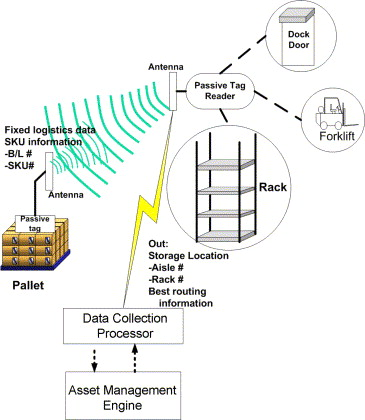
\includegraphics[width=0.5\textwidth]{../images/passive.jpg}	
		\caption{Modul proměnných logistických dat\cite{chow2006design}}
		\label{fig:passive}
\end{figure}

K \texttt{modulu proměnných logistických dat} se vztahují ultra-širokopásmové technologie \texttt{(UWB)}, které definují přenos proměnných logistických dat mezi čtečkou a tagem, jak je znázorněno na obrázku \ref{fig:uwb}. Tento modul obsahuje kolekci aktivních tagů, čtyři čtečky \texttt{UWB} a \texttt{Hub procesor} pro sledování polohy zdrojů. \texttt{UWB} aktivní tagy se skládají z interní baterie a krátkého \texttt{impulsového} vysílače umožňujícího vysílat na mnohem delší vzdálenost. \texttt{Tag} vydá krátkodobý \texttt{pulzní} signál několikrát za sekundu. \texttt{UWB} čtečky přijímají signály a posílají je do Hub procesoru. S logickým nastavením\texttt{triangulace} rozdílného čtení \texttt{UWB} čteček lze vypočítat přesné (x, y, z) souřadnice aktivního \texttt{tagu}. Přitom je koordinace zdrojů ve skladu přesně vypočítaná. Takové koordinace zdrojů budou předány \texttt{sledovacímu modulu zdroje} pro následné zpracování.\cite{chow2006design}


\begin{figure}[ht]
		\centering
		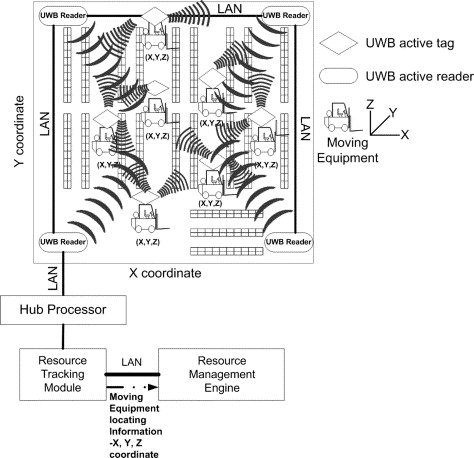
\includegraphics[width=0.6\textwidth]{../images/uwb.jpg}	
		\caption{Modul proměnných logistických dat\cite{chow2006design}}
		\label{fig:uwb}
\end{figure}




\subsection{Sledování}
\texttt{Modul sledování zdrojů} je server, který uloží všechny údaje aktivních \texttt{tagů} a poskytuje výkonné prostředí pro manipulaci s daty, filtruje a předává veškeré užitečné údaje řízení zdrojů pro formulování obchodní logiky a rozhodování. To je základem pro řízení zdrojů pro provádění činností včetně řízení zdrojů, plánování zdrojů, využívání a měření výkonnosti. Kromě výše uvedených funkcí, modul sledování je schopný převést data \texttt{UWB} na (x, y, z) souřadnice, které pak poskytují v reálném čase vizuální zobrazení přesného umístění zdroje na mapě skladu.\cite{chow2006design}

\subsection{Řízení}
\texttt{Modul řízení zdrojů} zpracovává data z aktivních \texttt{tagů} v reálném čase. Na základě těchto informací hledá optimální trasu a délku cesty k vyzvednutí zdrojů každým potenciálním manipulačním zařízením. V důsledku toho je vybráno zařízení nejvhodnější pro provedení úkolu.\cite{chow2006design}
	


\chapter{Popis zařízení}
	\section{Raspberry Pi}
		\texttt{Raspberry Pi (RPi)} je řada malých jedno deskových počítačů, vyvíjená ve Velké Británii.\\		
		Pro tento projekt se použije \texttt{Raspberry Pi 2 Model B}, číslovka v názvu určuje generaci a \texttt{model B} značí osazení \texttt{Ethernetovým portem} na rozdíl od \texttt{modelu A}.
		\texttt{RPi} má procesor \texttt{Broadcom BCM2836 ARM Cortex-A7 Quad Core} \texttt{700 MHz} lze přetaktovat na \texttt{900 MHz}, \texttt{1GB RAM}, 4x \texttt{USB 2.0}, \texttt{HDMI}, \texttt{4-pólový jack} a již zmiňovaný \texttt{10/100 Ethernet}. Přenosová rychlost \texttt{ethernetu} je velmi omezená, protože je napojený na \texttt{USB řadič}.\\
		V slotu \texttt{MicroSDHC} musí být \texttt{microSD karta}, protože zní se musí nabootovat operační systém.\\
		Na desce jsou ještě umístěny 2 řady \texttt{pinů}, takzvané \texttt{GPIO} viz. obrázek \ref{fig:gpio}.\\
		PRi neobsahuje \texttt{RTC (Real Time Clock)}, získávání aktuálního času se řeší pomocí \texttt{NTP (Network Time Protocol)}.
	

		\subsection{GPIO}
			\texttt{GPIO (General Purpose Input/Output)} je \texttt{40 pinů} umístěných na desce ve dvouch řadách. Číslování pinů je dvojího typu \texttt{BCM} a \texttt{BOARD}, u \texttt{BCM} se počítají jen nastavitelné piny, když to u \texttt{BOARD} se počítají všechny.
Mezi nenastavitelné piny patří napájení \texttt{5V} (\textcolor{red}{\textbf{červená}}), napájení \texttt{3V3} (\textcolor{orange}{\textbf{oranžová}}) a \texttt{zem} (\textbf{černá}) viz. obrázek \ref{fig:gpio} .	
		
		\begin{figure}[h]
   		 	\centering
			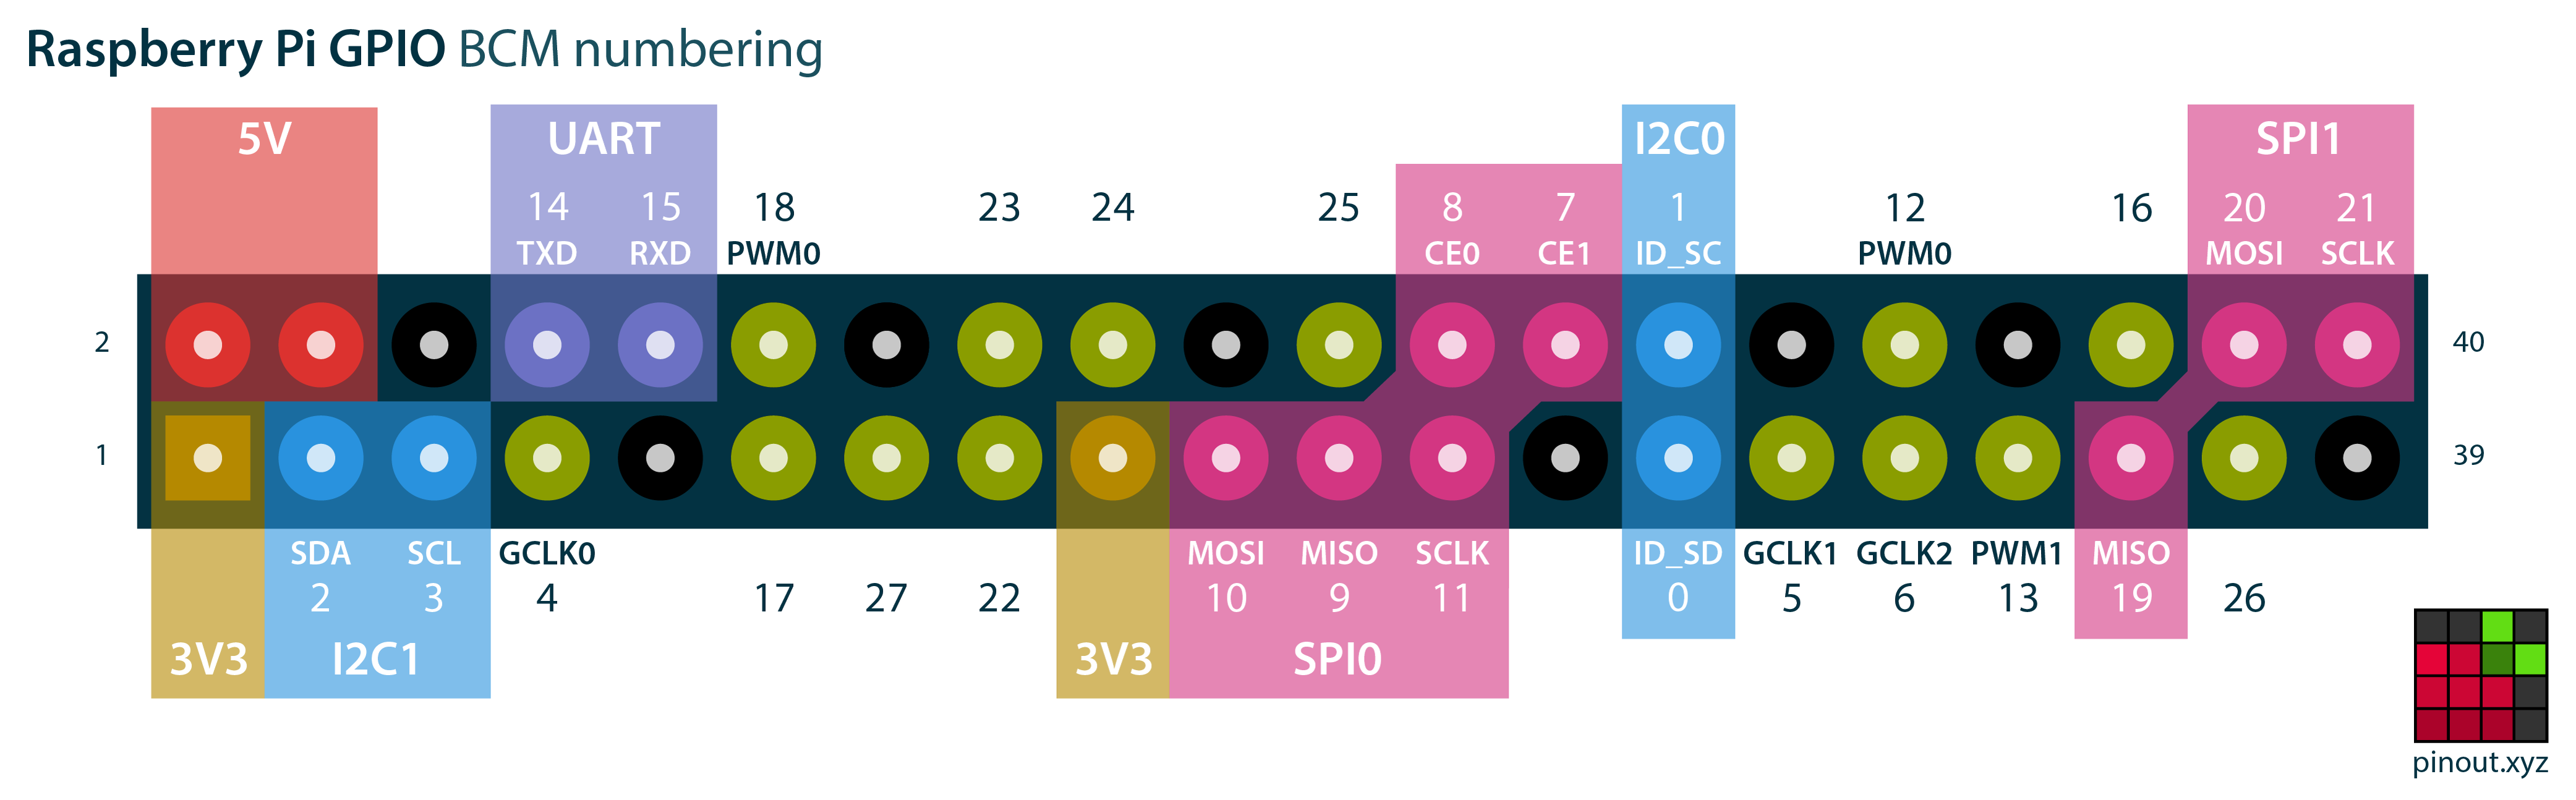
\includegraphics[width=1\textwidth]{../images/gpio.png}	
			\caption{Schéma \texttt{GPIO}}
    		\label{fig:gpio}
		\end{figure}		
		
		
		\subsection{Operační systémy}
			\subsubsection{Raspbian}
				\texttt{Raspbian} je operační systém založený na linuxové distribuci \texttt{Debian} a optimalizován pro hardware \texttt{Raspberry Pi}. Systém je vydáván ve dvou verzích Pixel a Lite, verze Pixel obsahuje navíc \texttt{GUI} a balíčky pro vývoj, což se promítlo na celkové velikost 4GB oproti Lite verzi s 1,5 GB. Pro většinu hlavních programujících jazyků je k dispozici knihovna pro ovládání \texttt{GPIO}.
			
			\subsubsection{Windows 10 IoT Core}
			Verze \texttt{Windows 10 IoT Core} je určena pro minipočítače typu \texttt{Raspberry Pi}. Systém je v raném vývoji a je na stránkách Microsoftu k dispozici zdarma.\\ Systém nemá uživatelské rozhraní. Spravuje se přes webové rozhraní nebo \texttt{Powershell} nebo na něm běží aplikace, která uživatelské rozhraní může mít. Spustit lze pouze \texttt{Universal Windows Platform (UWP)} aplikace, které je možné psát v \texttt{c\#}, \texttt{c/c++}, \texttt{Pythonu}, \texttt{Node.js} a \texttt{javascriptu}. Pro vývoj a nahrání \texttt{UWP} aplikace je zapotřebí mít \texttt{Visual Studio 2015}.

\newpage			
	\section{RFID}
\texttt{RFID} představuje technologii identifikace pomocí radiofrekvenčních vln. Jedná se v podstatě o generaci identifikátorů navržených (nejen) k identifikaci zboží, navazujících na systém \texttt{čárových kódů}. Identifikace a dohledatelnost je možná celosvětově, a to při dodržení standardu dat \texttt{EPC Global} a s využitím internetového rozhraní \texttt{EPC Global Network}. \texttt{EPC} o délce 96 bitů nabízí dostatečný číselný prostor 268 milionům výrobců produkujícím každý 16 milionů druhů výrobků (tříd), přičemž v každé třídě je prostor pro 68 miliard sériových čísel.\cite{dolevcek2010identifikace}

\subsection{Základní princip}
Technologie \texttt{RFID} pracuje na principu radaru. \texttt{Transpondéry (tagy)} mohou být jak aktivní, tak pasivní. Čtečka nejprve vysílá na svém nosném kmitočtu \texttt{elektromagnetickou vlnu}, která je přijata anténou pasivního \texttt{transpondéru}. \texttt{Indukované napětí} vyvolá elektrický proud, který je usměrněn a nabíjí \texttt{kondenzátor} v \texttt{transpondéru}. Uložená energie je použita pro napájení \texttt{logických} a \texttt{rádiových obvodů} transpondéru. Když napětí na \texttt{kondenzátoru} dosáhne minimální potřené úrovně, spustí se \texttt{logický automat} či \texttt{mikroprocesor} a \texttt{transpondér} začne odesílat odpověď čtečce. Vysílání \texttt{transpondéru} je realizováno zpravidla pomocí dvoustavové \texttt{ASK (Amplitude Shifting Key)} modulace, která je realizována změnou zakončovací impedance antény \texttt{transpondéru}. Odrazy, které vznikají změnou \texttt{impedance} antény, jsou detekovány čtečkou do \texttt{binární} podoby. Řízení komunikace a jednotlivých stavů komunikačního řetězce je definováno příslušnou \texttt{ISO normou}.\cite{dolevcek2010identifikace}

\subsection{Forma tagu}
\texttt{RFID tag} - paměťový \texttt{radiofrekvenční} čip nesoucí datovou informaci, který komunikuje bezkontaktně a bez přímé viditelnosti se snímačem - nejčastěji v podobě etikety nebo štítku. Provedení (tvar, rozměry, materiál) se mohou velmi lišit dle požadavků aplikace. \texttt{RFID tag} se skládá z vlastního čipu, antény, propojení a zapouzdření, případně baterie. Čip definuje kapacitu a typ \texttt{RFID tagu}, anténa stanovuje kvalitu příjmu a odesílání \texttt{radiofrekvenčního} signálu, zapouzdření ovlivňuje možnost použití v různých prostředích a životnost tagu.\cite{dolevcek2010identifikace}

\newpage
\begin{description}
\item [RFID Smart label]
- čip je umístěn na po tisknutelné etiketě s možností dalších informací (text, \texttt{čárový kód}) viz. obrázek \ref{fig:gpio}
\item [RFID wristband] - náramek na ruku obsahující \texttt{RFID} čip,  využití ve zdravotnictví k identifikaci osob.
\item [RFID karta] - čip může být zapouzdřen do plastové karty nebo předmětu typu klíčenky – např. k využití v platebních a docházkových systémech.
\item [RFID inlay] - zabudování čipu přímo do produktu, v případě kovového výrobku možnost oddělující vrstvy kvůli rušení.
\end{description}

\begin{figure}[ht]
   		 	\centering
			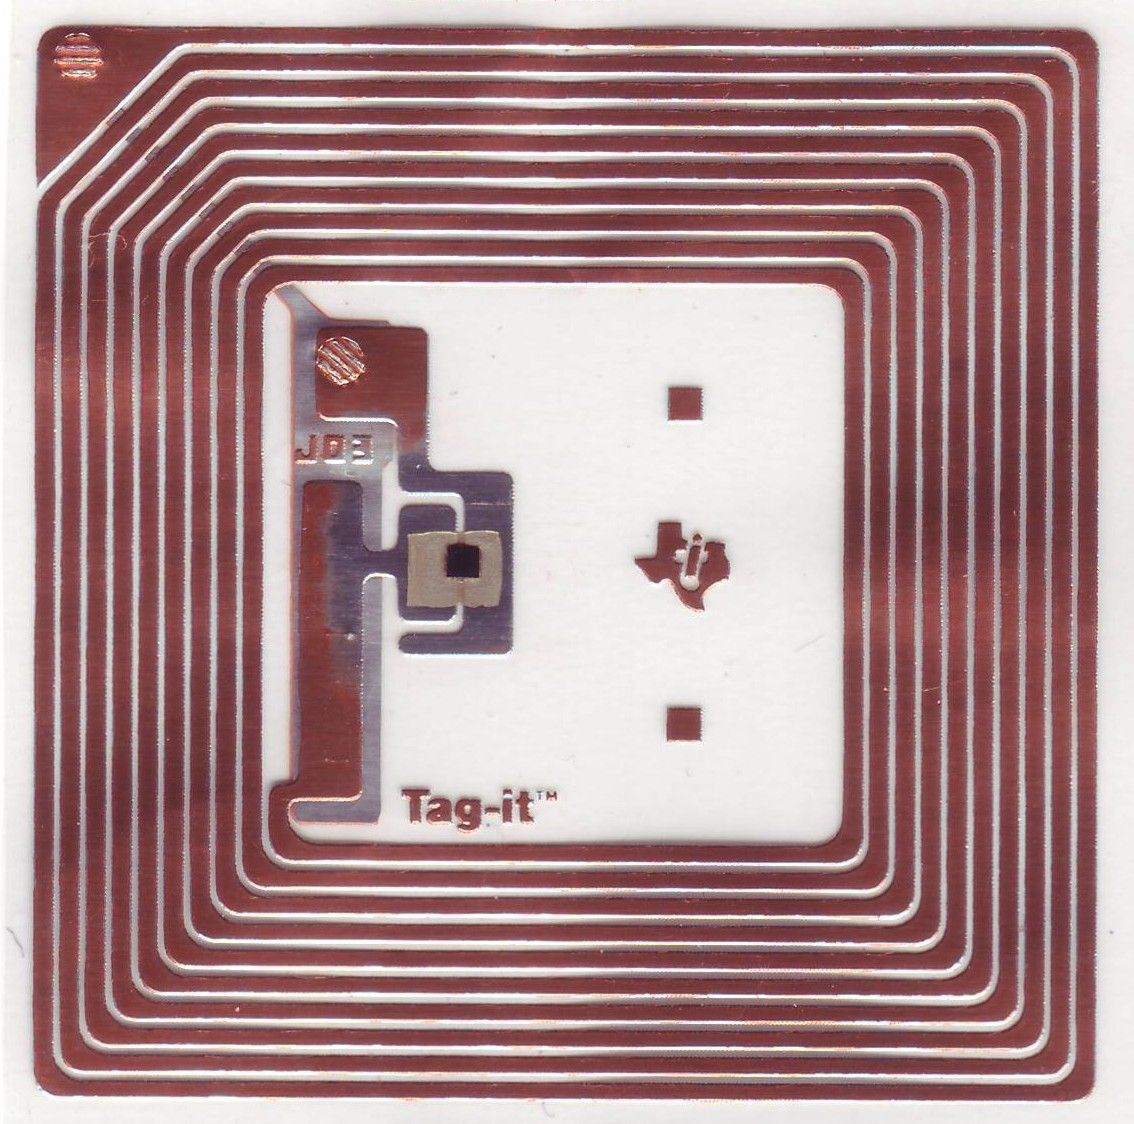
\includegraphics[width=0.6\textwidth]{../images/rfid_smart_label.jpg}	
			\caption{Pasivní HF RFID}
    		\label{fig:gpio}
		\end{figure}


\subsection{Frekvenční pásma}
Systémy \texttt{RFID} pracují s různými frekvencemi, která ovlivňuje rychlost čtení a zápisu, dosah signálu a prostor pokrytí atd.
Více informací v tabulce \ref{table:rfid_frekvence}

\begin{table}[ht]
\centering
\begin{tabular}{ c | c | p{5cm}}
 	\textbf{Frekvence} & \textbf{Dosah} & \textbf{Popis} \\ \hline\hline
    Nízká frekvence (LF) & \multirow{2}{*}{0,5 m} & \multirow{4}{5cm}{krátký dosah, velká anténa, pouze pro čtení, nízká přenosová rychlost, kovy a kapaliny nevadí} \\
    125–134 kHz &  & \\ 
    &  & \\ &  & \\ \hline
    
    Vysoká frekvence (HF) & \multirow{2}{*}{1 m} & \multirow{4}{5cm}{krátký dosah, velká anténa, pouze pro čtení, kapaliny znesnadňují čtení}  \\ 
	13,56 MHz &  & \\ 
	&  & \\ &  & \\ \hline       
	
    Velmi vysoká frekvence (UHF) & \multirow{2}{*}{3 m} &  \multirow{4}{5cm}{možnost číst i zapisovat, vysoká přenosová rychlost, nelze číst přes kapaliny }\\  
    860-930 MHz &  & \\ 
    &  & \\ &  & \\ \hline
    
    Mikrovlnná frekvence (MW) &  \multirow{2}{*}{10 m} & \multirow{4}{5cm}{možnost číst i zapisovat, vysoká přenosová rychlost, kapaliny a kovy příliš nevadí } \\
	2,54 a 5,8 GHz &  & \\ 
	&  & \\ &  & \\ \hline
\end{tabular}
\caption{Frekvenční pásma RFID}
\label{table:rfid_frekvence}
\end{table}

\newpage

\subsection{Zdroje napájení}
Čipy (\texttt{tagy}) se dělí na aktivní a pasivní podle toho, zda je možné informace z nich nejen číst (pasivní), ale i do nich zapisovat (aktivní). Aktivní jednotky pak musí disponovat vlastním zdrojem energie; ten obstarává miniaturní baterie. Jejich paměť pro zápis může dosahovat až 1 MB.\cite{dolevcek2010identifikace}

\subsubsection{Pasivní}
Pasivní zdroje jsou nejrozšířenější, nemají vlastní baterii, napájeny jsou polem snímače. Ten periodicky vysílá pulsy prostřednictvím antény do prostoru, čip využije přijímaný signál k nabití svého napájecího \texttt{kondenzátoru} a vyšle odpověď. Pasivní tagy mají různou vzdálenost čtení od 0,5 m do 10 m, dlouhou životnost čipu a používají metodu \texttt{RTF (reader talk first)}. V současné době jsou nejvíce rozšířeny pasivní čipy a to zejména kvůli své nenáročnosti na obsluhu a odolnosti, velikost paměti 64-256 bitů.\cite{dolevcek2010identifikace}
\subsubsection{Aktivní}
Aktivní zdroje mají vlastní baterii, jsou schopny vyslat svoji identifikaci. Používají se méně často než pasivní systém \texttt{RFID}. Jsou složitější, obsahují navíc i zdroj napájení a jsou schopny samostatně vysílat své identifikace - používají se proto pro aktivní lokalizaci.
Aktivní čipy vysílají samy své údaje do okolí \texttt{TTF (tag talks first)}, to umožňuje vlastní miniaturní baterie umístěná v čipu, která vydrží cca 1-5 let. Tyto čipy však kvůli baterii mají menší odolnost na teplotu a je nutné provádět výměnu baterie. Aktivní čipy mají vzdálenost čtení až 100 m, velikost paměti na čipu může dosahovat až 100 kb.\cite{dolevcek2010identifikace}


\subsection{Čtečka}
Snímače neboli čtečky \texttt{RFID} jsou zařízení, která dokáží zachytit vysílání aktivního nebo pasivního tagu. Čtečka nemusí pouze informace zachycovat, ale také může do \texttt{tagu} zapisovat. Čtečka používá pro vysílání a přijímání signálu anténu, která může být integrovaná nebo externí. Základním požadavkem na čtečku je schopnost zpracovat obrovské množství dat. Čtečky musí poznat již jednou přečtené \texttt{tagy} a odstranit odrazy signálů tagů od pevných překážek a musí zvládnout současně načíst velký počet \texttt{tagů}. S tím souvisí schopnost paralelně načítat \texttt{tagy} v relativně krátkém časovém intervalu.\cite{dolevcek2010identifikace}	
	
	
	
	
	
	
	
	
	
	
	
	
	
	
\chapter{Návrh řešení}




		\section{Komunikace}
		
		\subsection{MQTT}
	
		\subsection{REST API}
	
	\section{Databáze}
		\subsection{MongoDB}
		\subsection{Modely}
	
	
\chapter{Server}

	\section{Platforma}
		nodejs

	\section{Autorizace}
		
	\subsection{MQTT}		
	\subsection{API}
		\subsubsection{Basic Auth}
		\subsubsection{JSON Web Token}
		\subsubsection{OAuth 2.0}
			
		
	\section{Použité knihovny}
		npm	
	
		\subsection{Mosca}
		\subsection{Restify}
		\subsection{Mongoose}
		\subsection{Bunyan}
		\subsection{Swagger}
		\subsection{Passport}
		\subsection{Swagger}
		
	
\chapter{Čtečka RFID}
	požadavky na čtečku

	\section{Sestavení}

	\section{Platforma}
		linux Raspbian, python
	
	\section{Komunikace}
	
	\section{Použité knihovny}
		\subsection{RPi.GPIO}
		\subsection{RC522}
			https://github.com/ondryaso/pi-rc522
		\subsection{Eclipse Paho}
			http://www.eclipse.org/paho/
		\subsection{SPI-Py}
			https://github.com/lthiery/SPI-Py

\chapter{Mobilní aplikace}
	požadavky na mobilní aplikaci

	\section{Platforma}
	
	\section{Komunikace}
		

	\section{Použité knihovny}
		\subsection{Retrofit}
		\subsection{Butter Knife}

\chapter{Testovnání a zhodnocení výsledků}	

\chapter{Možnosti rozšíření}

\chapter{Závěr}


\chapter*{Přehled zkratek}


\bibliographystyle{csplainnatkiv}
{\raggedright\small
\bibliography{literature}
}

\chapter*{Postup nasazení}
\addcontentsline{toc}{chapter}{Postup nasazení}

\chapter*{Uživatelský manuál}
\addcontentsline{toc}{chapter}{Uživatelský manuál}

\chapter*{Obsah přiloženého CD}
\addcontentsline{toc}{chapter}{Obsah přiloženého CD}


\end{document}